\chapter{Methoden}

\section{Quarzkristall-Mikrowaage}
Eine Möglichkeit, die Masse  eines aufgedampften Materials
zu bestimmen, ist die Änderung der Eigenfrequenz 
einer angeregten Quarzplatte (Quartz Crystal Microbalance, "QCM") zu untersuchen.
Durch die Vergrößerung der schwingenden Masse $\symup{\Delta}m$ ändert sich die Frequenz $\symup{\Delta}f$ nach der Sauerbrey Gleichung \cite{sauerbrey1959verwendung},
was auf den linearen Zusammenhang

\begin{equation}
        \symup{\Delta}f = -\symup{C} \cdot \symup{\Delta}m
\end{equation}

führt. Der Faktor $\symup{C}$ bezeichnet eine Kalibrierungskonstante. Aus der aufgedampften Masse lässt sich über die Dichte des Materials 
die gewachsene Schichtdicke und damit die Aufdampfrate in $\si{\angstrom\per\minute}$ bestimmen.
Diese gibt einen Anhaltspunkt für die spätere Aufdampfrate auf der untersuchten Probe, 
weicht aber um einen konstanten Faktor von der tatsächlichen Rate ab. 
Eine Ursache dafür sind unterschiedliche Adsorptionsraten des Quarzkristalls und der untersuchten Probe.




\section{LEED und IV-LEED}

Zur Strukturbestimmung in Festkörpern eignen sich allgemein Beugungsmethoden mit Teilchen, deren Wellenlänge in der Größenordnung der 
zu untersuchenden Struktur liegt. Bei der Beugung niederenergetischer Elektronen (Low Energy Electron Diffraction, "LEED") werden Elektronen 
genutzt, deren Energien im Bereich $E=50$-$200$\,eV liegen, sodass sie zum Einen passend für eine atomare Auflösung sind und zum Anderen durch ihre geringe mittlere freie Weglänge 
eine oberflächensensitive Methode bilden. 

Dabei trifft ein Elektronenstrahl aus einer Elektronenkanone senkrecht auf die Probe, welcher dort gebeugt und anschließend 
zurück auf einen  Fluoreszenz-basierten Leuchtschirm trifft. 
Inelastisch gestreute Elektronen werden durch Gitter mit passender Gegenspannung herausgefiltert.
Hinter den Gittern werden die elastisch gestreuten Elektronen zum Leuchtschirm hin beschleunigt.
Die dort entstehenden Beugungsreflexe werden mit einer Kamera aufgenommen.

\begin{SCfigure}
        \centering
        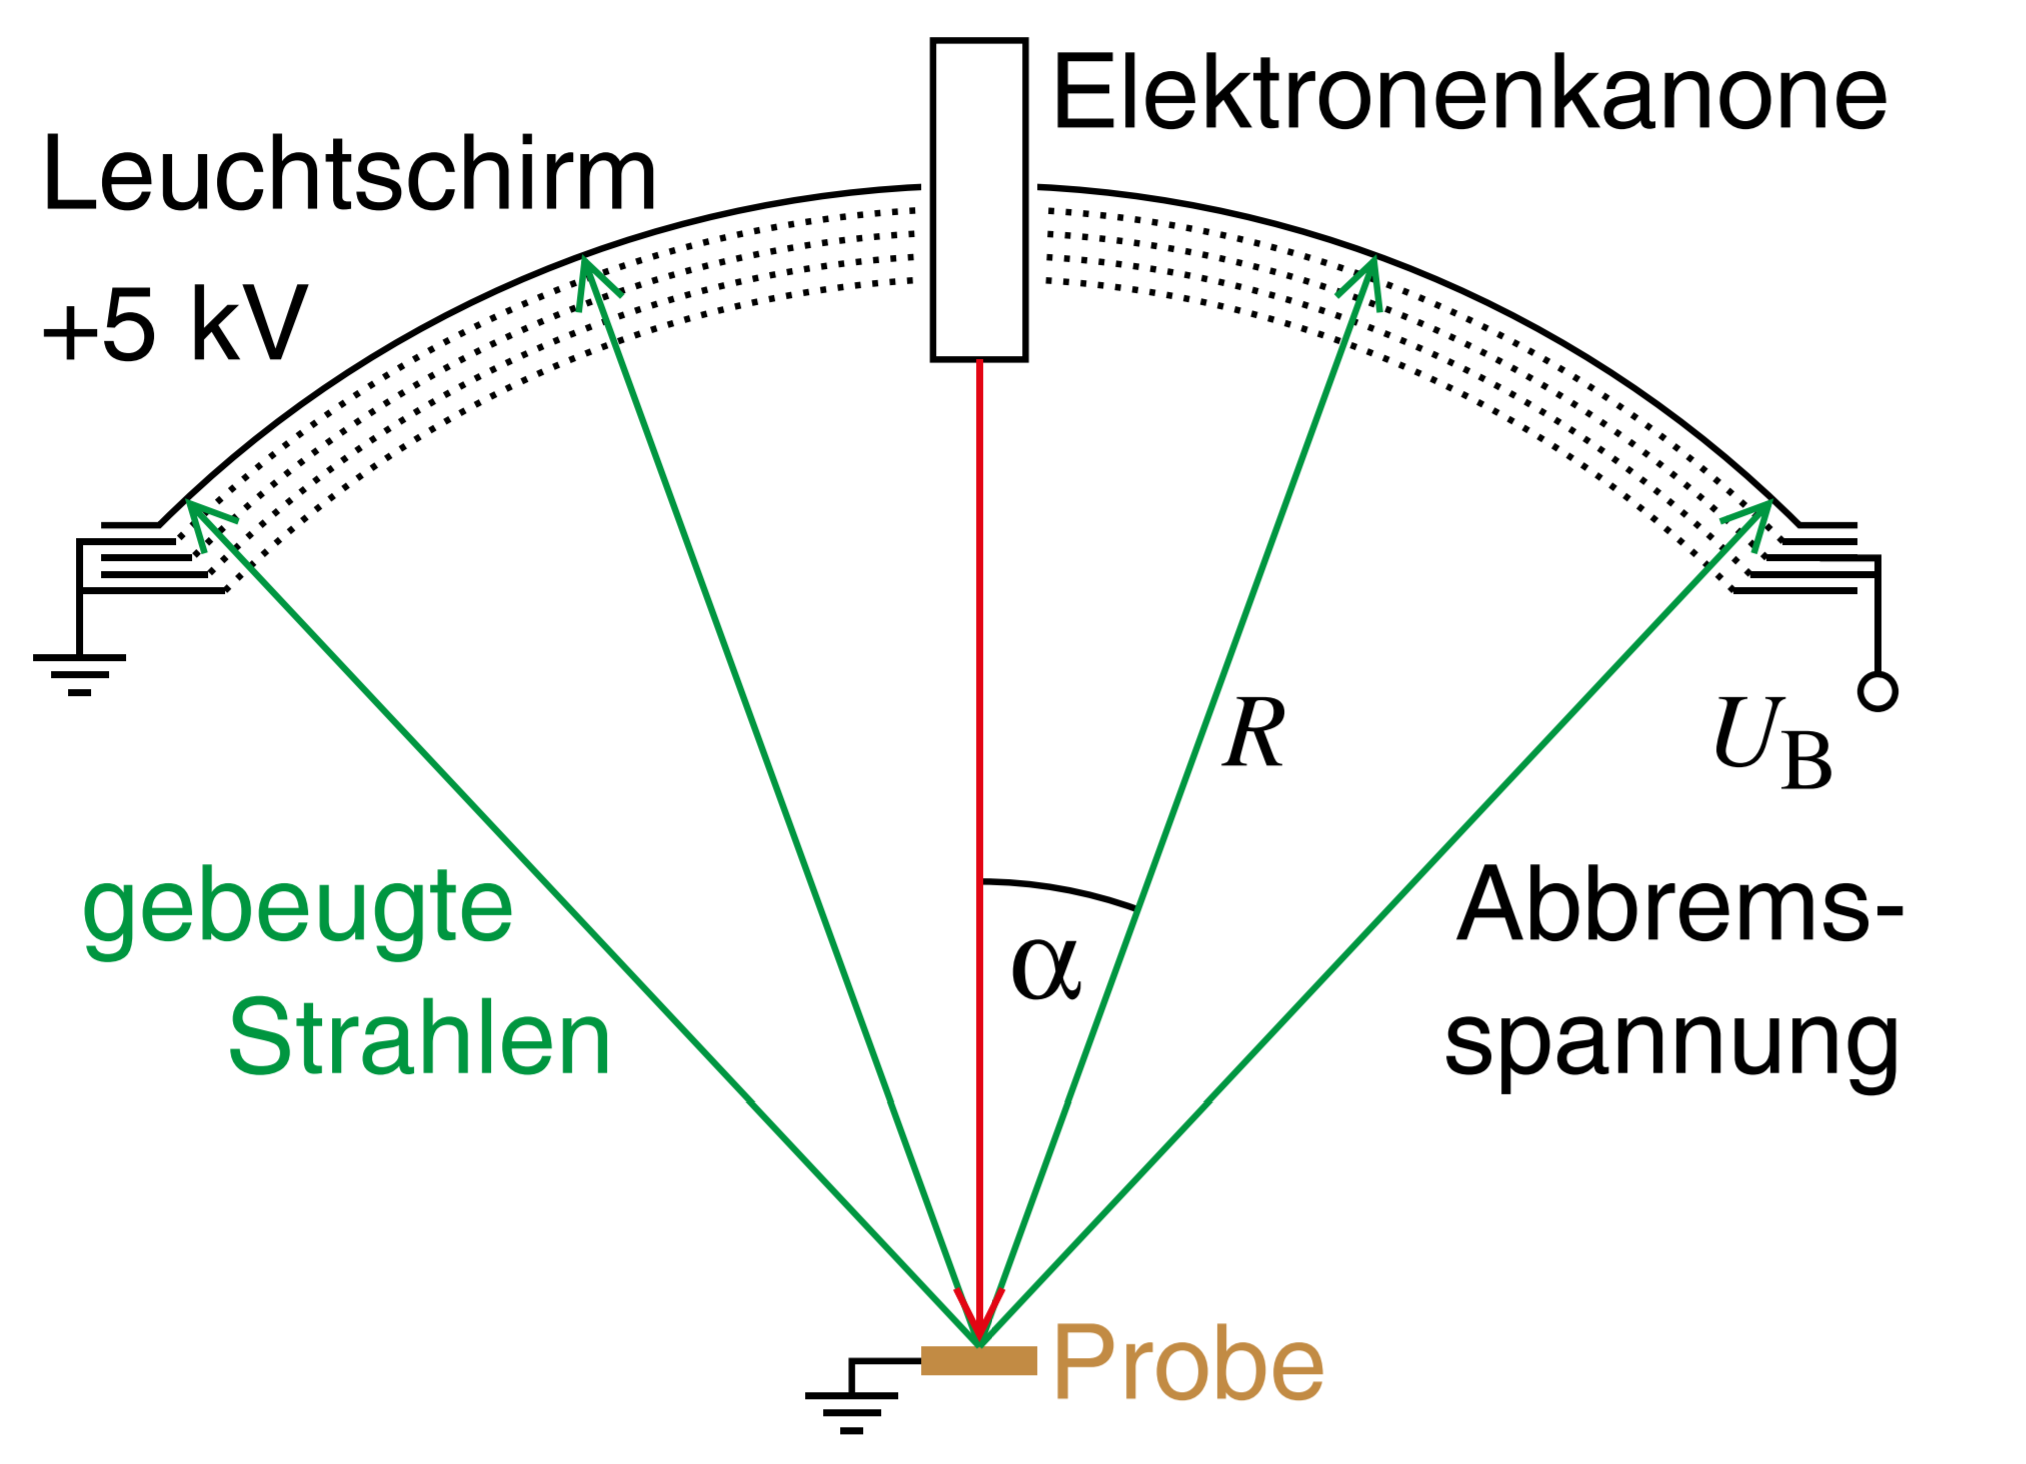
\includegraphics[width=0.5\linewidth]{Plots/LEED_Schema.png}
        \caption{Schematische Darstellung einer LEED-Optik. In grün ist die Bahn der elastisch gestreuten Elektronen zu sehen,
        welche unter dem Winkel $\alpha$ an der Probe gebeugt werden und auf den gekrümmten Leuchtschirm mit Radius $R$ treffen.
        Am Gitter liegt eine Abbremsspannung $U_{\symup{B}}$ an, um inelastisch gestreute Elektronen auszufiltern \cite{fauster}.}
        \label{fig:LEED_Schema}
\end{SCfigure}

Die Beugungsintensität $I$ hängt vom Formfaktor $F$ und vom Gitterfaktor $G$ ab
\begin{equation}
        I=|F|^2\cdot |G|^2.
        \label{eq:LEED}
\end{equation}

Es gilt nur dann $G\neq 0$, wenn die Laue-Bedingung $\symup{\Delta}\vec{k}_{||}=\vec{g}_{hk}$ für den Impulsübertrag in senkrechter Richtung erfüllt ist.
$\vec{g}_{hk}$ bezeichnet hier einen diskreten reziproken Gittervektor.
Es treten also nur bestimmte Beugungsreflexe auf, die durch die Bezeichnung ($hk$) identifiziert werden.
Die Beugungsreflexe geben ein Bild des reziproken Raums der Oberfläche wieder
und sind charakteristisch für die Oberflächenstruktur der Probe.
Ist die Ordnung der Oberfläche zum Beispiel durch Fremdatome gestört, treten weitere Streueffekte auf und
die Reflexe verlieren an Schärfe.

Nach Gleichung \ref{eq:LEED} wirken sich unterschiedliche Strukturen direkt auf die Reflex-Intensität aus, 
weshalb  diese zur Charakterisierung eines Materials verwendet werden kann.
Dafür werden so genannte IV-Kurven genutzt, die die Intensitätsverläufe einzelner Reflexe in Abhängigkeit der Energie 
wiedergeben.
\newpage

\section{MEED}
Die Beugung mittelenergetischer Elektronen (Medium-Energy Electron Diffraction, "MEED") kann in einem Reflektionsaufbau \ref{fig:MEEDS} 
genutzt werden, um die Anzahl der Monolagen während des Wachstums zu bestimmen.

\begin{figure}[H]
        \centering
        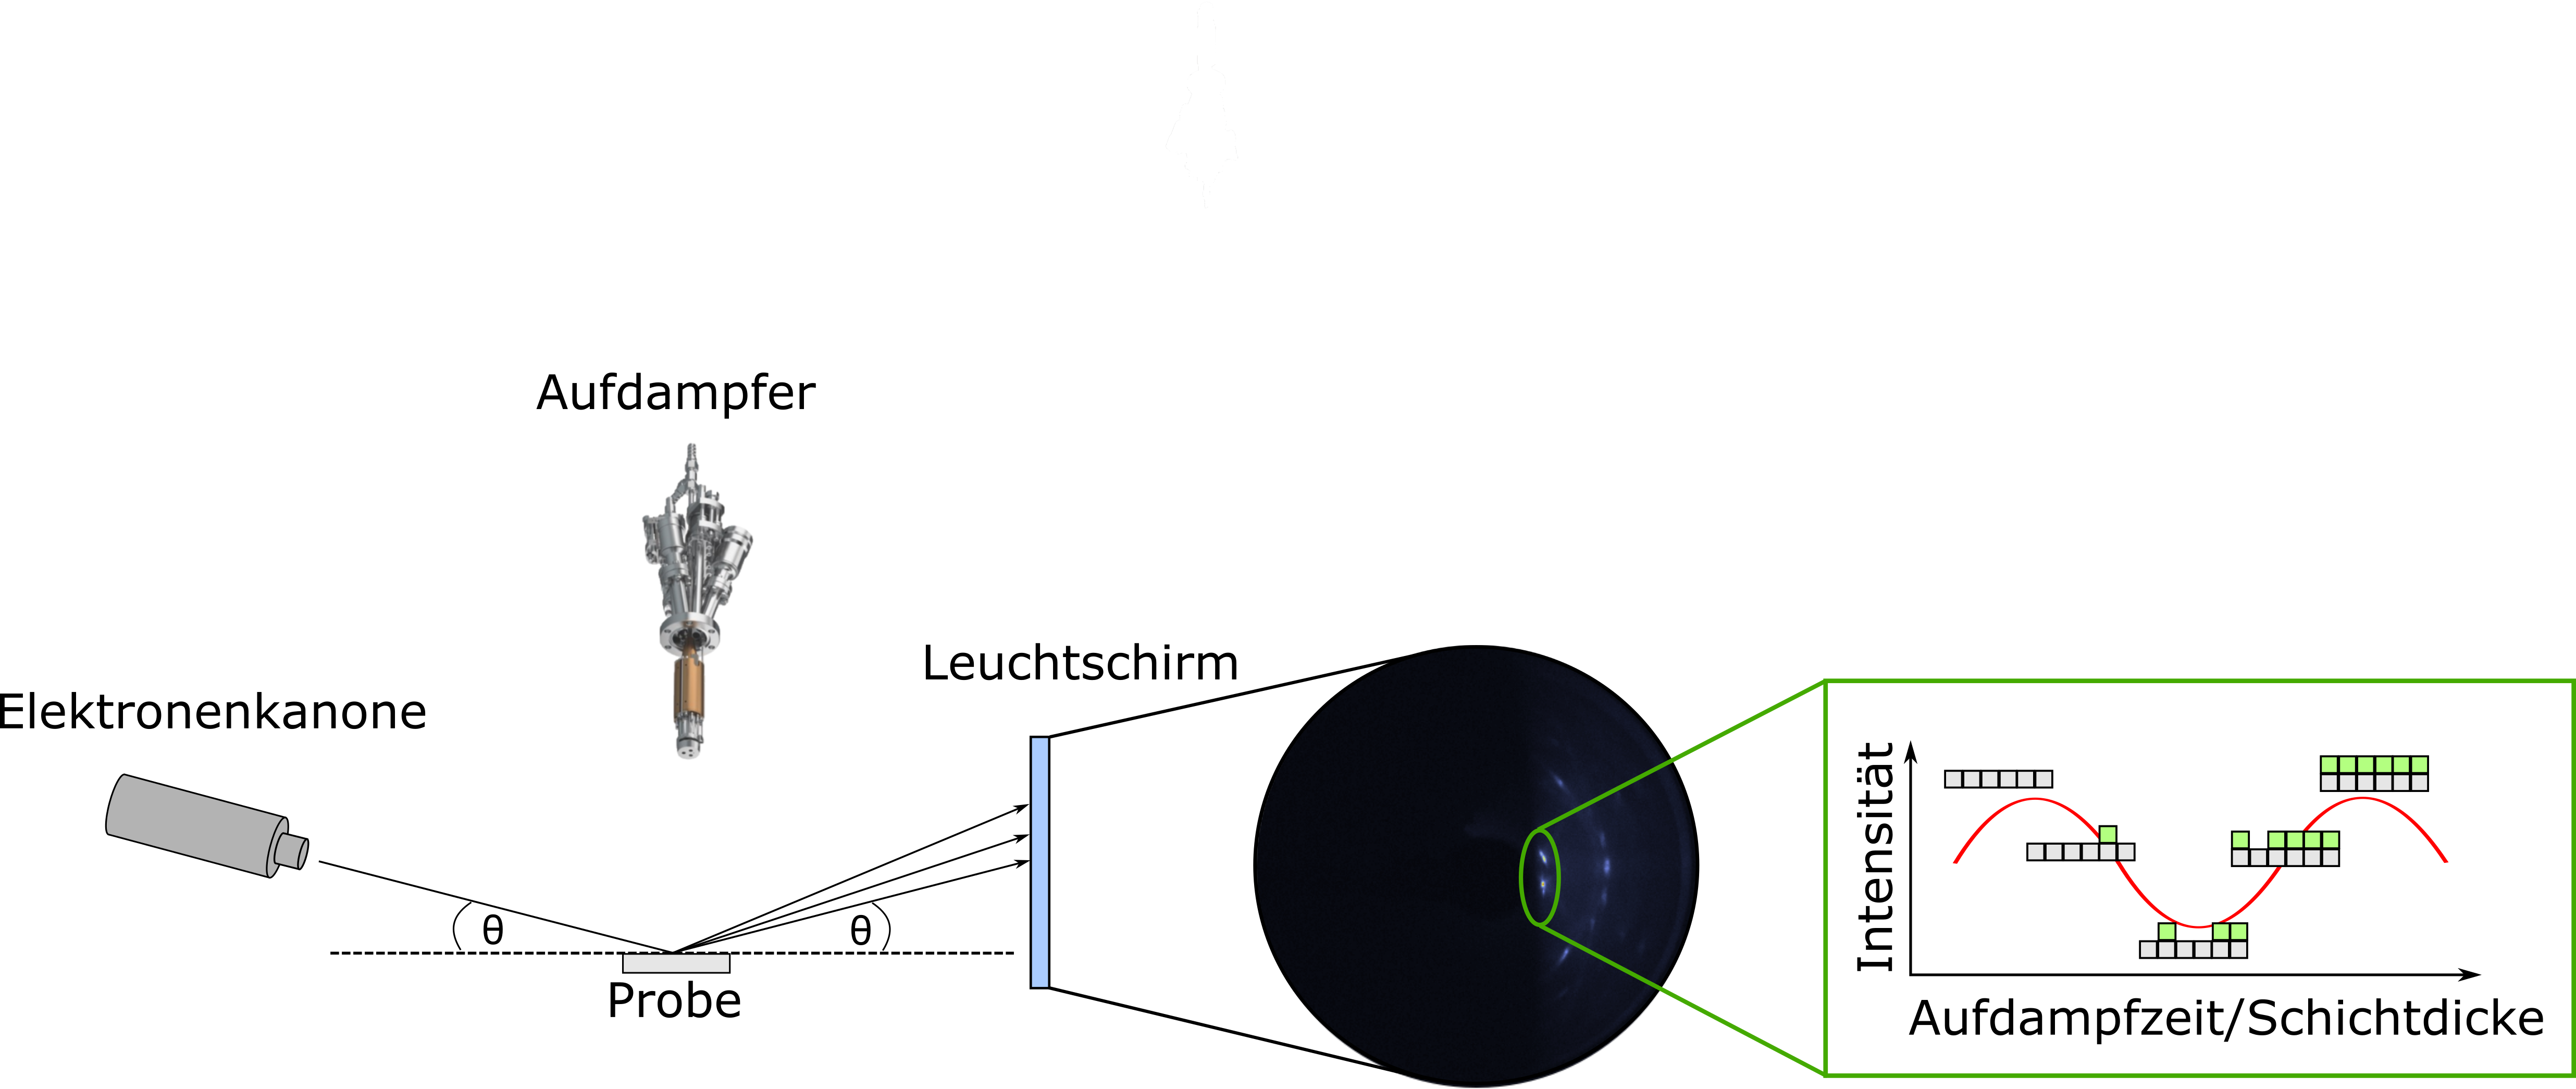
\includegraphics[width=\linewidth]{Plots/MEED_3.pdf}
        \caption{Schematische Darstellung der MEED-Methode im Reflexionsaufbau. Die Elektronenkanone befindet sich gegenüber des
                Leuchtschirms, der Elektronenstrahl kann so in einem flachen Winkel $\Theta$ auf die Probe treffen.
                Dort werden die Elektronen wie bei der LEED-Methode elastisch gestreut und bilden ein Beugungsbild am Leuchtschirm.
                Befindet sich der Aufdampfer \cite{FOCUS} wie abgebildet vor der Probe, kann das Beugungsbild 
                während des Wachstums beobachtet werden. Die Intensität der Beugungsreflexe oszilliert mit der Schichtdicke.
                Mit freundlicher Genehmigung von David Janas.}
        \label{fig:MEEDS}
\end{figure}

Die Intensität der Beugungsreflexe oszilliert dabei in Abhängigkeit der Struktur der Oberfläche.
Die beste Ordnung und demnach die höchste Intensität besteht bei einer abgeschlossenen vollen Monolage.
Bei einem lagenweisen Wachstum kann nun die Bildung einer neuen Lage zunächst durch einen Abfall der Intensität beobachtet werden, 
auf den ein erneuter Anstieg folgt, bis die neue Monolage vollständig ist. Anhand der Anzahl der Intensitätsmaxima lässt sich so die
Anzahl der Monolagen beim Wachstum dünner Schichten bestimmen \cite{neave1983dynamics}. 




\newpage
\section{Augerelektronenspektroskopie}
\label{sec:Auger}
Eine oberflächensensitive Methode zur quantitativen Elementanalyse einer Probe ist die Augerelektronenspektroskopie (Auger Elektron Spectroscopy, "AES").
Mit Hilfe der mittleren freien Weglänge von Elektronen in den entsprechenden Systemen lässt sich aus den Peak-Verhältnissen eines Auger-Spektrums außerdem die Schichtdicke bestimmen.

Wird in einem Atom ein Elektron aus einer inneren Schale z.B. durch Elektronenstrahlung herausgelöst,
wird das entstehende Loch durch ein Elektron einer äußeren Schale aufgefüllt. 
Wenn die dabei frei werdende Energie an ein weiteres Elektron übertragen wird,
kann dieses den Festkörper verlassen und wird Augerelektron genannt.
Dessen Energie ist dabei abhängig von den beteiligten Energieniveaus des Atoms, und somit elementspezifisch.
Wird die Anzahl der detektierten Elektronen in Abhängigkeit ihrer Energie aufgetragen, bilden sich bei den entsprechenden Energien 
charakteristische Peaks, wie beispielhaft in Abbildung \ref{fig:Auger-BSP} gezeigt. Die Intensität wird dabei in differentieller Form dargestellt,
um die Peaks vor dem Untergund inelastisch rückgestreuter Elektronen und Sekundärelektronen hervorzuheben.

\begin{figure}[H]
        \centering
        \includegraphics[width=0.7\linewidth]{Plots/plotAuger2_Layout.pdf}
        \caption{Augerspektrum einer dünnen MgO-Schicht auf Fe(100). Die Elementzugehörigkeiten der gemessenen Peaks sind entsprechend gekennzeichnet.}
        \label{fig:Auger-BSP}
\end{figure}


Um unterschiedliche elementspezifische Faktoren, wie die Wahrscheinlichkeit für einen Augerzerfall,
bei den relativen Peak-Verhältnissen einbeziehen zu können,
werden relative Sensitivitäten $S_{\symup{i}}$ des Elements i definiert, welche empirisch bestimmt werden \cite{davis-1978}.
Die für das zu untersuchende System wichtigen Sensitivitäten von Fe, O und Mg sind in Tabelle \ref{tab:AugerS} aufgetragen.
Die Elementkonzentration $c_{\symup{i}}$ kann so mit der Gleichung 

\begin{equation}
        c_{\symup{i}}=\dfrac{{I_{\symup{i}}}/{S_{\symup{i}}}}{\sum_{\symup{j}}{I_{\symup{j}}}/{S_{\symup{j}}}}
        \label{eq:AugerK}
\end{equation}

bestimmt werden, wobei $I_{\symup{i}}$ die Peak-Intensität bezeichnet. Die Summe läuft über alle vorhandenen Elemente j \cite{fauster}.

\begin{table}[H]
        \centering
        \begin{tabular}{S | S}
          \toprule
          {$\symup{Element}$} & {$S_{\symup{i}}$}\\
          \midrule
          $\symup{Fe \:(651\,eV)}$ & {$0,2$}\\
          $\symup{O \:(503\,eV)}$ & {$0,5$} \\
          $\symup{Mg \:(1174\,eV)}$ & {$0,1$}\\
          \bottomrule
        \end{tabular}
        \caption{Relative Sensitivitäten $S_{\symup{i}}$ der untersuchten Elemente Fe, O und Mg \cite{davis-1978}.}
        \label{tab:AugerS}
\end{table}
Um die Schichtdicke aus Augerspektren zu bestimmen, ist es wichtig, die mittleren freien Weglängen $\lambda$ von Elektronen bei den Energien zu kennen, 
bei denen die charakteristischen Peaks auftreten. In der Literatur lassen sich verschiedene mittlere freie Weglängen finden,
wovon einige in Tabelle \ref{tab:AugerM} aufgeführt sind.

\begin{table}
        \centering
        \begin{tabular}{c| c c c c}
          \toprule
          Energie & Gries \cite{gries1996universal} & Tanuma et al. \cite{tanuma1994calculations}& Akermann et al. \cite{akkerman1996inelastic}& Seah et al. \cite{seah1979quantitative}\\
          \midrule
          {$651\,\si{\eV}$} & {$14,62\,\si{\angstrom}$} & {$16,35\,\si{\angstrom}$} & {$15,48\,\si{\angstrom}$} & {$18,9\,\si{\angstrom}$}\\
          {$503\,\si{\eV}$} & {$12,70\,\si{\angstrom}$} & {$13,65\,\si{\angstrom}$} & {$12,69\,\si{\angstrom}$} & {$16,7\,\si{\angstrom}$}\\
          {$1174\,\si{\eV}$} & {$22,55\,\si{\angstrom}$}& {$25,34\,\si{\angstrom}$}& {$24,72\,\si{\angstrom}$}& {$23,5\,\si{\angstrom}$}\\
          \bottomrule
        \end{tabular}
        \caption{Mittlere freie Weglängen bei den relevanten Energien in MgO \cite{Wachstum}.}
        \label{tab:AugerM}
      \end{table}


\begin{equation}
        \dfrac{I_{\symup{A}}}{I_{\symup{S}}}=\dfrac{S_{\symup{A}}\cdot \left( 1-\symup{exp}\left( -\dfrac{d}{0,74\cdot \lambda_{\symup{A}}} \right) \right) }  {S_{\symup{S}}\cdot \symup{exp} \left( -\dfrac{d}{0,74 \cdot\lambda_{\symup{S}}} \right) }
        \label{eq:Auger-V}
\end{equation} 

Gleichung \ref{eq:Auger-V} stellt einen Zusammenhang zwischen dem Augerpeak-Verhältnis des Adsorbats $I_{\symup{A}}$ zum Substrat $I_{\symup{S}}$ und der Schichtdicke $d$
des Absorbats her \cite{Wachstum}. 
\newpage


\section{Experimentelles Setup}

\begin{SCfigure}
        \centering
        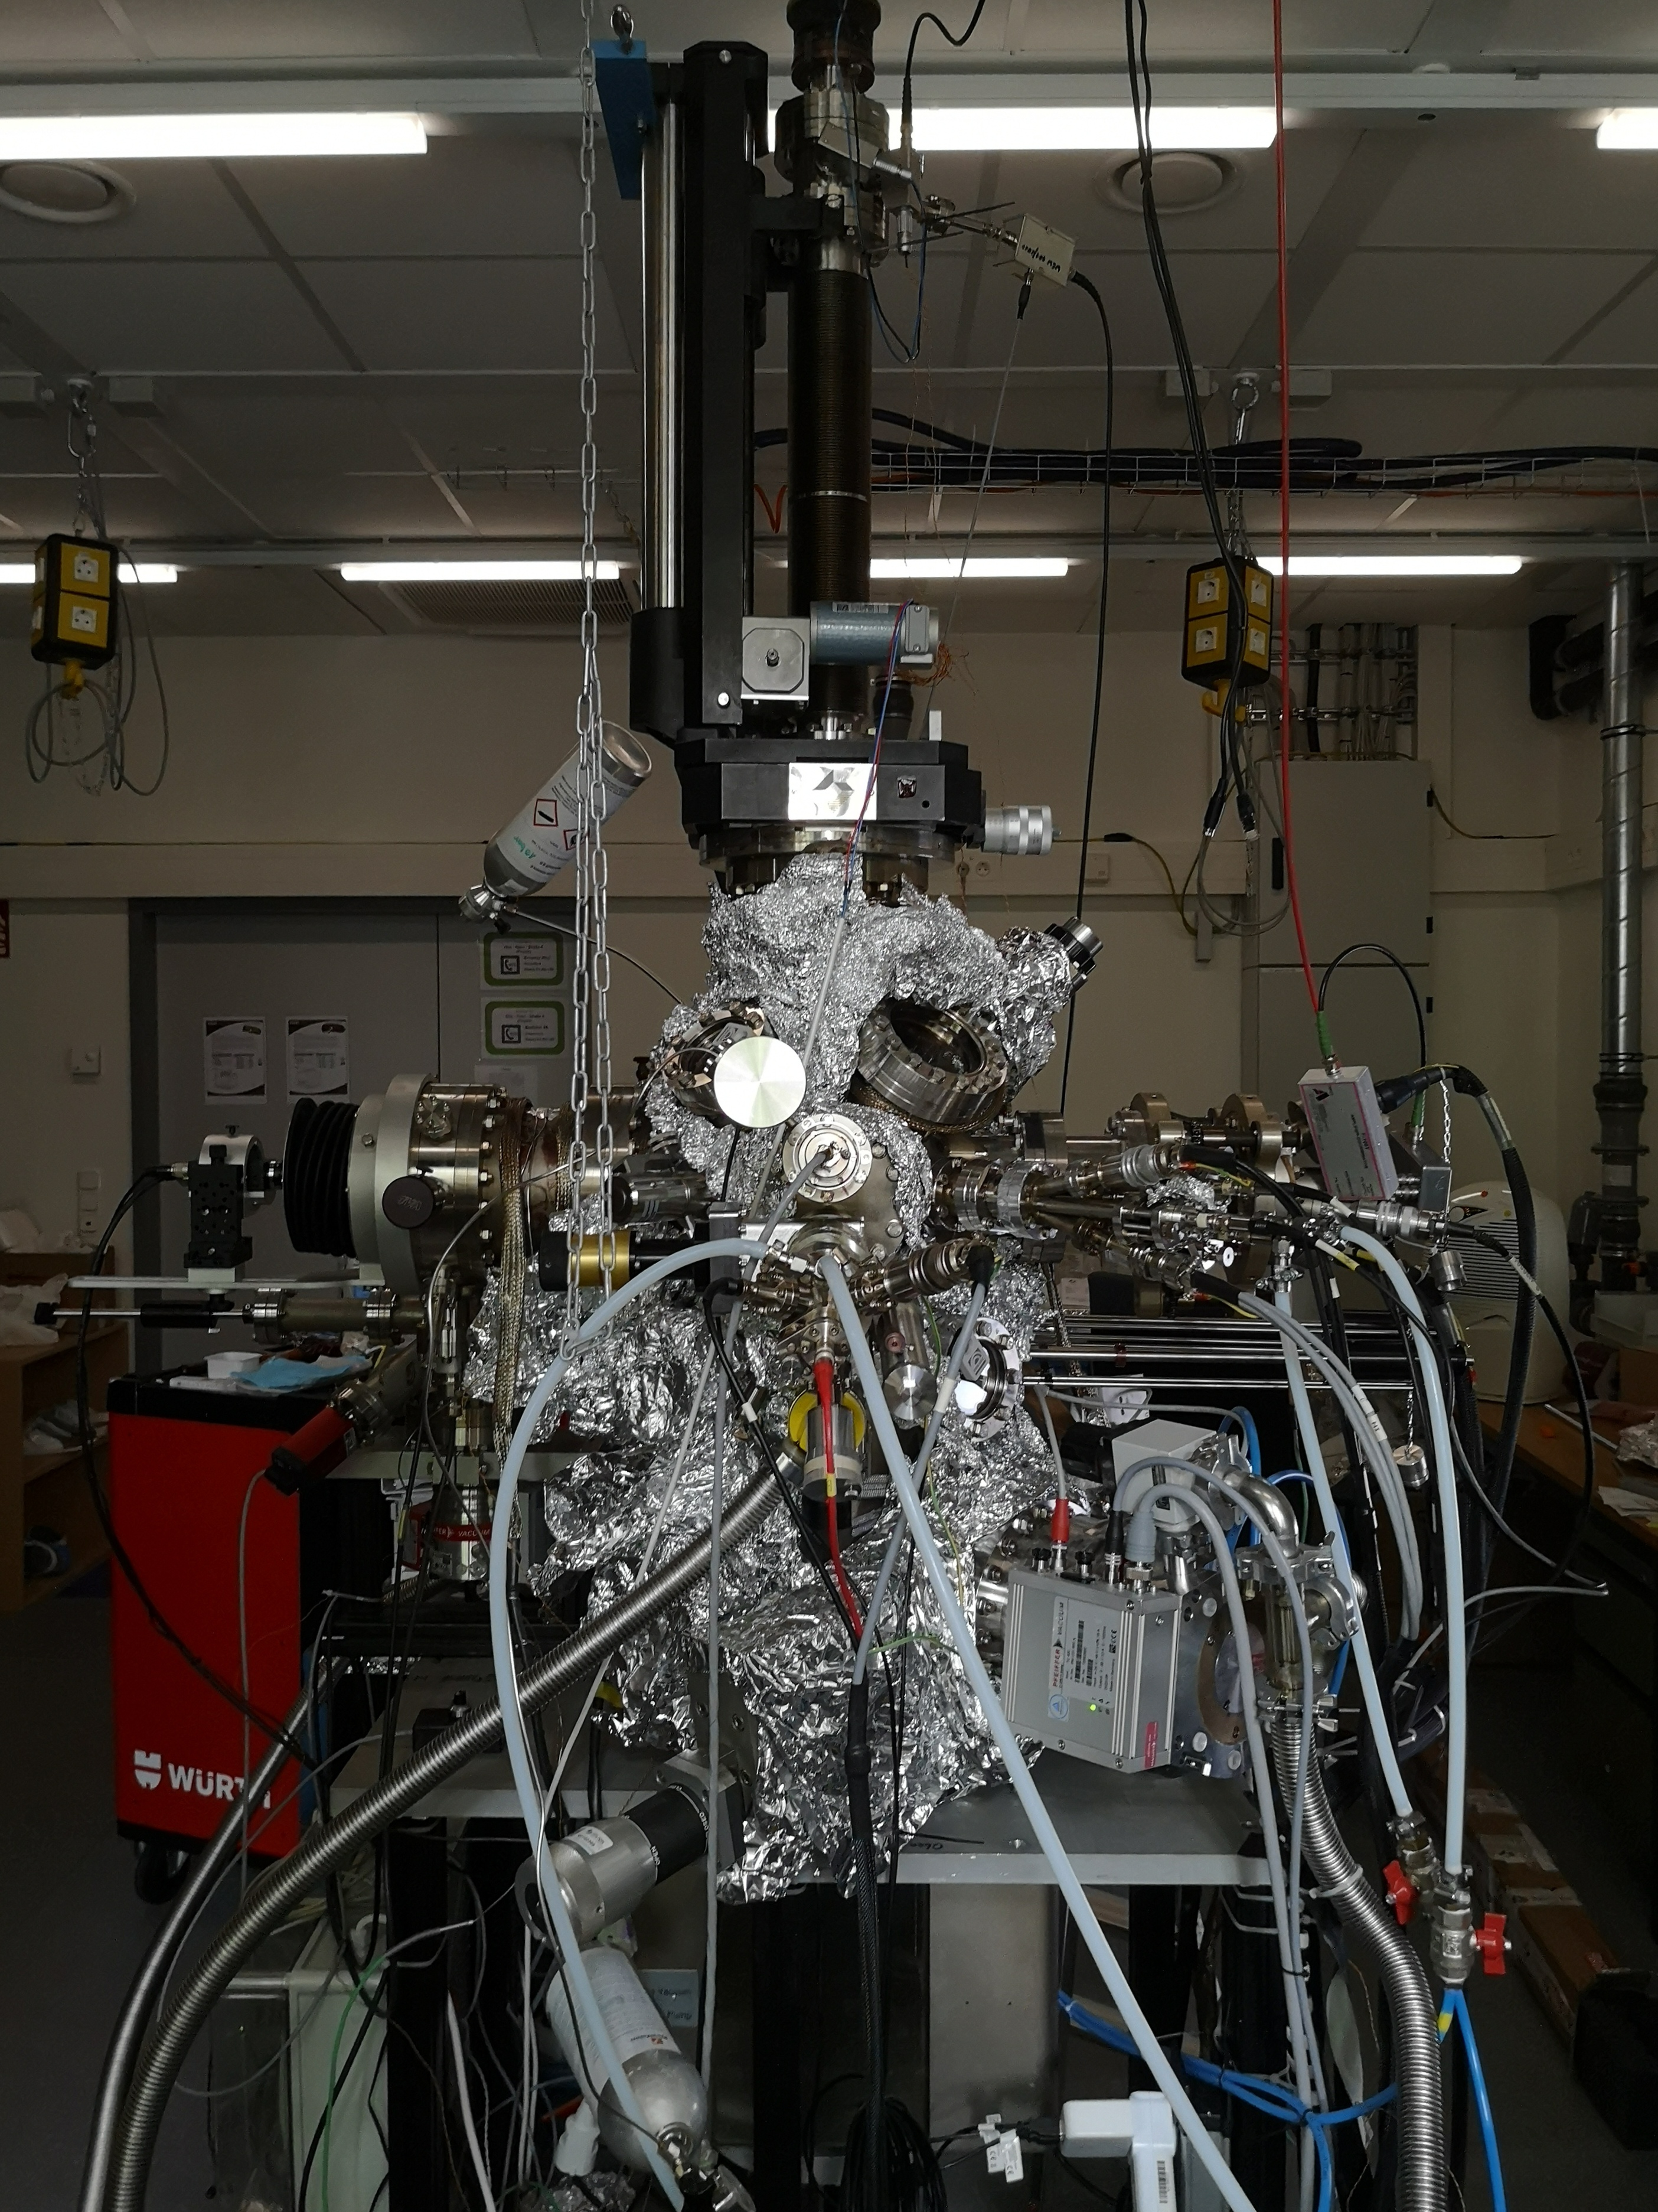
\includegraphics[width=0.6\linewidth]{Plots/BILD_PREP.pdf}
        \caption{Gezeigt ist die verwendete Präperationskammer. Beschriftet sind die Komponenten des Reflektions-MEED Aufbaus.}
        \label{fig:BILD_PREP}
\end{SCfigure}

Das Wachstum wurde in einer Ultra-Hoch Vakuum (UHV) Kammer durchgeführt, die auf das Wachstum und die Analyse dünner Schichtsysteme ausgelegt ist.
Der Basisdruck in der Kammer liegt in der Größenordnung von $p=6\cdot 10^{-11}\,\si{\milli\bar}$.
Zur ständigen Druckmessung wird dabei ein Ionisations-Vakuummeter verwendet.
In die Kammer können über Leckventile $\symup{Ar}^+$-Ionen sowie $\symup{O_2}$-Moleküle 
eingelassen werden. 

Die $\symup{Ar}^+$-Ionen werden dabei zum Reinigen der Probe mittels ioneninduzierter Zerstäubung (sputtering) verwendet.
Sie können durch eine angelegte Spannung unter einem Winkel auf die Probe beschleunigt werden und tragen durch Stöße Oberflächenatome ab.
Anschließendes Heizen der Probe mit einem Heizwiderstand sorgt für die Desorption weiterer Verunreinigungen sowie eine Neuordnung der 
Oberfläche durch zusätzliche thermische Energie.
 Die Temperatur wird mit einem Thermoelement gemessen, welches sich leicht entfernt von der Probe befindet, weshalb 
eine kleine Differenz zur tatsächlichen Temperatur der Probe vorliegt.

Die Probe ist in der Kammer durch einen Manipulator frei translatierbar und zudem um $360\,\si{\degree}$ um die z-Achse rotierbar.
Am Manipulator ist außerdem eine QCM befestigt, die in der Höhe und  Tiefe versetzt zur Probenhalterung angebracht ist.

Das Magnesium wird aus Pellets mit $99,99\,\si{\percent}$ Reinheit aus einem Molybdän-Tiegel aufgedampft.
Der Aufdampfer steht dabei in einem Winkel von $90\,\si{\degree}$ zum LEED-Schirm und zur Elektronenkanone des AES, was MEED-Messungen während des Aufdampfens ermöglicht.
Für unterschiedliche Winkel zwischen Probe und LEED-Schirm stellen sich verschiedene Beugungsordnungen ein, welche in Abbildung \ref{fig:MEED-Bilder} zu sehen sind.



\begin{figure}[H]
    \centering
    \subfloat[][]{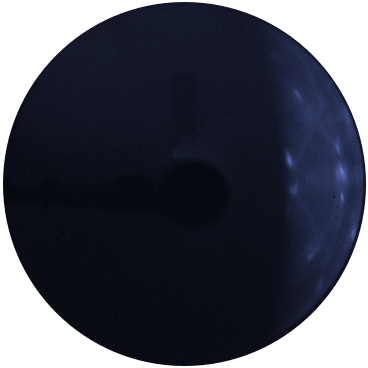
\includegraphics[width=0.28\linewidth]{Plots/MEED_103_degree.png}}%
    \qquad
    \subfloat[][]{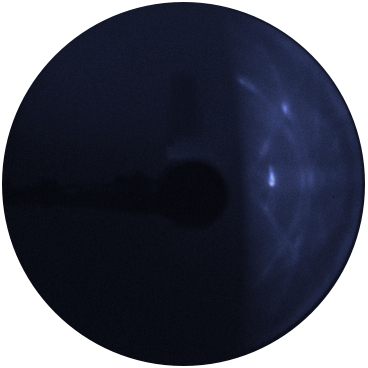
\includegraphics[width=0.28\linewidth]{Plots/MEED_109_degree.png}}%
    \qquad
    \subfloat[][]{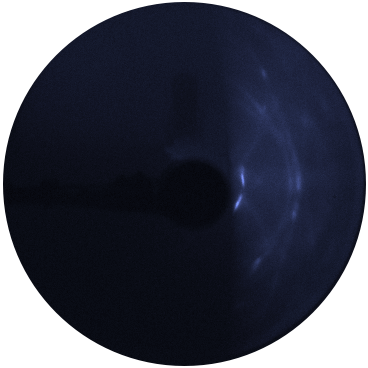
\includegraphics[width=0.28\linewidth]{Plots/MEED_113_degree.png}}%
    \caption{Bilder des LEED-Schirms mit MEED-Einstellungen für verschiedene Winkel zwischen Probe und Schirm. 
            (a) zeigt einen Winkel von $\Theta=13\,\si{\degree}$, (b) einen Winkel von $\Theta=7\,\si{\degree}$ und (c) einen Winkel von $\Theta=3\,\si{\degree}$ zwischen Probe und Schirm.}%
    \label{fig:MEED-Bilder}
  \end{figure}


